\documentclass[12pt,a4paper]{article}
\usepackage[utf8]{inputenc}
\usepackage[french]{babel}
\usepackage[T1]{fontenc}
\usepackage{amsmath}
\usepackage{amsfonts}
\usepackage{amssymb}
\usepackage{graphicx}
\usepackage{url}
\usepackage[usenames,dvipsnames]{xcolor}
\usepackage[colorlinks=false,urlbordercolor=white,linkbordercolor=white]{hyperref}
\usepackage[left=2cm,right=2cm,top=2cm,bottom=3cm]{geometry}
\usepackage{fancyhdr}
\usepackage{lmodern}
\usepackage{listings}
\pagestyle{fancy}
\usepackage{titlesec}
\usepackage[abs]{overpic}
\usepackage{tabularx}
\usepackage{times}
\usepackage{graphicx}

% gestion de la police sans-serif (helvetica, équivalent arial) :
% décommenter les deux lignes suivantes
%\usepackage{helvet}
%\renewcommand{\familydefault}{\sfdefault}

% Definition de l'affichage du code
\lstset{breaklines=true,basicstyle=\footnotesize\ttfamily,frame=single, numbers=left
%,backgroundcolor=\color{lightgray}
}

% Definition des couleurs
\definecolor{titreColor}{RGB}{0,58,128}  % Marine
\definecolor{stitreColor}{RGB}{0,158,224}  % Ocean
\definecolor{auteurColor}{RGB}{0,58,128}     % Marine
\definecolor{texteColor}{RGB}{164,196,0}     % Prairie

% Definition du sommaire
\usepackage[tight]{shorttoc}
\newcommand{\sommaire}{\shorttoc{Sommaire}{2}}

% Definition des chapitres
\titleformat{\section}
{\color{titreColor}\normalfont\Large\bfseries\sffamily}
{\color{titreColor}\thesection}{1em}{}

\titleformat{\subsection}
{\color{stitreColor}\bfseries\sffamily}
{\color{stitreColor}\thesubsection}{1em}{}

%Données de titre et d'auteur pour la page de garde
\newcommand{\titre}{Projet USACT}
\newcommand{\sousTitre}{Diagramme des cas d'utilisation}
\newcommand{\auteur}{Jérémy DAMEY}
\newcommand{\dateModif}{\today}


\begin{document}
%Supprime les veuves et orphelines
\widowpenalty=10000
\clubpenalty=10000
\raggedbottom 

%entete
\fancyhead{}
\renewcommand{\headrulewidth}{0pt}
%pied de page
\fancyfoot{}
\fancyfoot[C]{\sffamily\thepage}
\fancyfoot[L]{\textcolor{titreColor}{\sffamily\textbf{IRSTEA} - Centre de Bordeaux\\}
\fancyfoot[R]{\textcolor{auteurColor}{\sffamily\auteur{}}\\{\sffamily\dateModif{}}}
\textcolor{stitreColor}{\sffamily 50, avenue de Verdun, Gazinet\\
33612 CESTAS Cedex }}
\fancyfoot[R]{\sffamily\author{}}

% Insertion du logo, du titre et du sous-titre
\begin{minipage}{0.2\linewidth}

\includegraphics[width=3.06cm,height=9.57cm,keepaspectratio]{Image/logo_irstea}%
\end{minipage}
\hspace{0.1cm}
\begin{minipage}{0.8\linewidth}
\LARGE\flushleft \color{titreColor}{\bfseries\sffamily\titre{}}\\
\large\flushleft \color{stitreColor}{\bfseries\sffamily\sousTitre{}}
\end{minipage}

\vspace{1cm}
\begin{center}
\bf 
\color{titreColor}
\LARGE{Introduction}
\end{center}
Initialement créée pour collecter les conflits sur le Bassin d’Arcachon, avec une difficulté relative à la définition de ce qu’est un « conflit »,  car c’est un  objet complexe qui évolue dans le temps, l’espace, via les acteurs impliqués dont les revendications parfois multiples. L’étude des conflits s’appuie sur une méthodologie bien particulière développée par Torre et al. (2010). \newline
\underline {Petite information :} Torre, A., et al., Comment évaluer et mesurer la conflictualité liée aux usages de l'espace ? Eléments de méthode et de repérage. \newline \newline
Elle est basée sur l’utilisation de trois sources de données complémentaires :
\begin{description}
\item[–	La Presse Quotidienne Régionale  (PQR) :] pour accéder à une information locale détaillée. 
\item[–	Les entretiens auprès d’experts :] pour recueillir des informations auprès d’experts locaux, impliqués ou non dans les conflits. Construction d’une grille d’entretien commune. 
\item[–	Les relevés de contentieux :] permettant de recenser les conflits qui font l’objet d’un  traitement juridique. Ces données sont issues de la base Lamyline (pour éviter toute erreur, les noms de variables et les modalités de la base Lamyline sont conservés dans USACT). \newline
\end{description}


Initialement créée sous ACCESS, elle a été migrée vers un serveur de base de données en PostGreSQL. L’interface de saisie est alors devenue inadaptée et l’enjeu est donc de faciliter l’accès aux données via le développement de différents modules dans une application permettant aux chercheurs impliqués dans un projet, sur une zone d’étude bien délimitée, d’accéder aux données, en lecture et en écriture. \newline \newline
Pour des explications plus générale, vous pouvez regarder le schéma ci-dessous qui représente les cas d'utilisation important pour bien modéliser le projet Usact. \newline
Nous avons donc 2 acteurs dont un acteur interne à savoir le chercheur et l'autre acteur est un acteur externe à savoir l'organisme. \newline
Nous allons maintenant voir l'influence de ces 2 acteurs sur chacun des cas d'utilisation à l'aide du schéma ci-dessous.

\clearpage
\begin{figure}
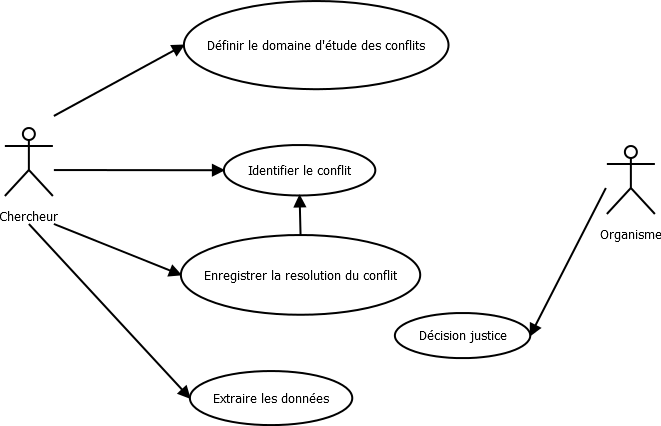
\includegraphics[width=17cm,height=20cm,keepaspectratio]{Image/casUtilisation}%
\caption{Diagramme des cas d'utilisation}
\end{figure}

\vspace{1cm}
\section{Chercheur}
Le chercheur est l'utilisateur de l'application. Chaque chercheur à le même rôle au sein de l'application. Il n'y a aucune différence par rapport aux droits d'accès. La seule différence se situe au niveau du domaine que nous allons voir dans la seconde partie.

\section{Définir le domaine d'étude des conflits}
Tout d'abord, commençons par recontextualiser le domaine d'étude avec une définition. \newline
\underline{Domaine d'étude :} c'est un ensemble de peuplements susceptibles d'être soumis à un même scénario de gestion. \newline
Au sein de l'IRSTEA, il y a 3 domaines : Arcachon, Marseille et l'Île de la Réunion. 
Le chercheur doit sélectionner le domaine d'étude le plus proche de son lieu de travail pour pouvoir accéder au contenu de l'application par la suite. Il est obligé de sélectionné le domaine qui lui a été attribué sinon, il n'aura pas accès au contenu de l'application, la connexion lui sera tout simplement refusée. 

\section{Identifier le conflit}
Nous allons tout d'abord commencé par une définition car un conflit est notion qui n'est pas facile a assimilé. \newline
\underline{Conflit :} Un conflit (et plus précisément son expression) est identifié via l’une des trois sources de données précédemment citées (article, entretien, contentieux). Ensuite, il convient de déterminer les caractéristiques du conflit. L’étape suivante s'intéresse aux parties prenantes du conflit, les acteurs : « fiche identité » de l’acteur et son intervention dans le conflit avec ses revendications, ses modes d’actions et les solutions proposées. \newline 
\underline{Plus précisément, comment est identifié un conflit :}
\begin{description}
\item[Source de données :] informations sur la source de données
\item[Matérialité du conflit :] informations sur le bien support, l’objet du conflit
\item[Genèse et déroulement du conflit :] période, localisation, résolution 
\item[Acteurs du conflit :] informations sur les personnes (physiques et/ou morales) qui participent au conflit
\item[Interventions des acteurs dans le conflit :] rôle de l’acteur, lien avec la matérialité du conflit, motifs de revendication et types d’arguments invoqués, mode d’action, solution proposée \newline \newline
\end{description}



L'identification d'un conflit correspond à la déclaration du conflit en lui-même, c'est-à-dire à sa création, peu import s'il est existant car on le référence par sa date d'apparition.
Quand on identifie un conflit, il faut également identifier le ou les acteurs ainsi que les sources parlant de ce conflit.

% Insertion d'une tabulation
\begin{description}
\item[Identifier les acteurs :] Ces acteurs sont ceux qui sont à l'origine du conflit, autrement dit cela peut-être n'importe qui ayant un quelconque problème. Par exemple cela peut-être un ostréiculteur ayant un problème avec la construction d'un ilot juste à coté de ses tuiles ...
\item[Identifier les sources :] Comme pour les domaines, il y a également 3 sources qui nous apportent différentes informations sur le conflit en question, à savoir la presse (à travers les journaux), les entretiens avec les experts (apport d'informations supplémentaires par rapport à ce qui a été dit dans la presse) et enfin le contentieux (à savoir la décision qui a été prise au tribunal suite à la contestation d'un des acteurs).
\end{description}

\section{Enregistrer la résolution du conflit}
En parallèle, des solutions sont élaborées pour résoudre les conflits en cours. Elles peuvent être trouvées pendant le conflit mais également avant, à savoir que ce conflit-là pouvait avoir été prévu à l'avance et que par conséquent la solution est déjà existante.

\section{Extraire les données}
L'utilisateur aura également la possibilité de pouvoir consulter les informations se rapportant aux conflits qu'il aura auparavant sélectionnés. Il pourra également savoir si le conflit est résolu ou pas (ou en cours de résolution).

\section{Organisme}

\section{Décision justice}

% Insertion du sommaire
% \sommaire
%\tableofcontents

% Debut effectif du texte

\end{document}